\documentclass[a4paper, 12pt]{IEEEtran}
\usepackage[utf8]{inputenc}
\usepackage[margin = 0.75in, top = 0.25in]{geometry}
\usepackage[style = ieee]{biblatex}
\usepackage{blindtext}
\usepackage{wrapfig}
\usepackage{graphicx}
\usepackage{hyperref}

\title{EEE-351 Term Project Proposal \\ Electromagnetic Suspension System}
\author{Tuna Alikaşifoğlu, Yiğit Berk Üçüncü, Berk Yaşar Yavuz}
\date{\today}
\graphicspath{{images/}}
\bibliography{bibliography}
\hypersetup{colorlinks = true, allcolors = black}

\begin{document}
\maketitle

\section{PROJECT DESCRIPTION}
In this term project, the aim is to build a system that demonstrates the fundamental concepts that are covered in the course EEE-351. For this purpose, a literature review is conducted, in order to come up with a suitable project proposal. In this process, we came across with the topic electromagnetic suspension, which fascinated us as a group. Electromagnetic suspension is a system that ``provides both additional stability and maneuverability by performing active roll and pitch control during cornering and braking, as well as eliminating road irregularities, hence increasing both vehicle and passenger safety and drive comfort''~\autocite{active_suspension}. However, this system manages to achieve this task by constantly altering the strength of a magnetic flux density via earnest feedback loop, which is too complex just to demonstrate basic electromagnetics concepts. Thus, we decided to implement the given system with a passive control mechanism, i.e., using two repelling magnets (see Fig.~\ref{fig:suspension}). In addition, 

Explain the concepts.

What we will going to do for this project~\autocite{emt_textbook}.

\begin{figure}[h]
    \centering
    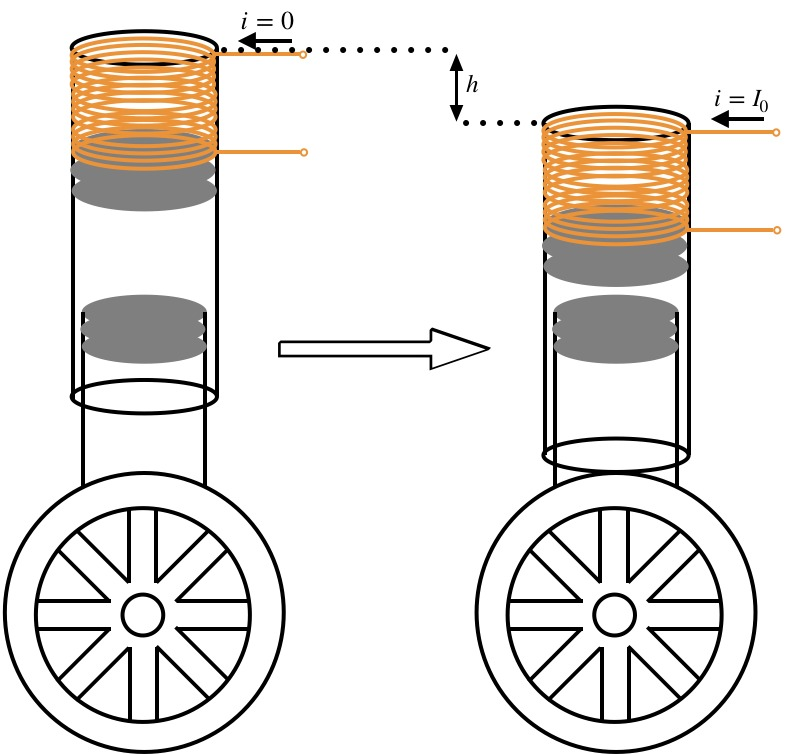
\includegraphics[width=0.48\textwidth, height=0.25\textheight, keepaspectratio]{suspension.jpeg}
    \caption{Designed Suspension System}\label{fig:suspension}
\end{figure}

\section{WORK PLAN}
Firstly we calculated the magnetic flux density that we can obtain by flowing current through a solenoid and the resulting attraction and repulsion force when we put this solenoid in an external magnetic field caused by permanent magnets. Once calculations showed that we can obtain enough force for our purposes, we made an experiment to see if our calculations are realistic and we observe that they are agreed each other. After being convinced that we can hold our test car on the air along syringe axis by only magnetic force we are planning to make use of permanent magnets as a passive suspensions and we will try to change its height by applying additional magnetic field by flowing current through solenoid as depicted in Fig.~\ref{fig:suspension}. Finally, we are planning to control all these things such as changing the height of all four wheels independently from each other with a microcontroller via bluetooth.


\section{LIST OF EQUIPMENT}

\begin{itemize}
    \item Neodymium Magnets
    \item Syringes
    \item Handmade Solenoids (Wound by 0.5mm Copper Wire)
    \item Motor Driver with H-Bridge (LN298N)
    \item Power Source (Li-Po Battery or Power Supply)
    \item Microcontroller (Arduino or Counterpart)
    \item Bluetooth Module (HC05 or Counterpart)
    \item Toy Car Chassis and Wheels
\end{itemize}

\printbibliography{}

\end{document}